\subsection{Onda completa de puente}
Este rectificador utiliza cuatro diodos \textbf{1N4007} conectados como un
puente y conectados a una resistencia de $10[\text{k}\Omega]$, como se muestra
en la \textbf{figura~\ref{circuito04}}.

\begin{figure}[!h]
\centering
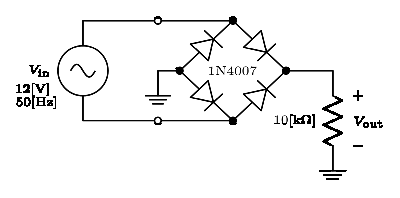
\includegraphics[scale=1.1]{diagramas/04.onda_completa1.eps}
\caption{Rectificador de onda completa con puente.}
\label{circuito04}
\end{figure}

Los valores positivos del voltaje de entrada polariza directamente a dos diodos
y polariza inversamente a los dos diodos restantes, mientras que los valores
negativos del voltaje hace el camino contrario por los diodos del circuito, lo
que genera la señal de onda completa con el doble de la frecuencia del voltaje
de entrada.

\subsubsection{Simulación}
Se utilizó el software \emph{Quite Universal Circuit Simulator.} versión 23.3.1
para la simulación del rectificador de onda completa, este puede verse en la
\textbf{figura~\ref{simulacion04}}.

\begin{figure}[!h]
\centering
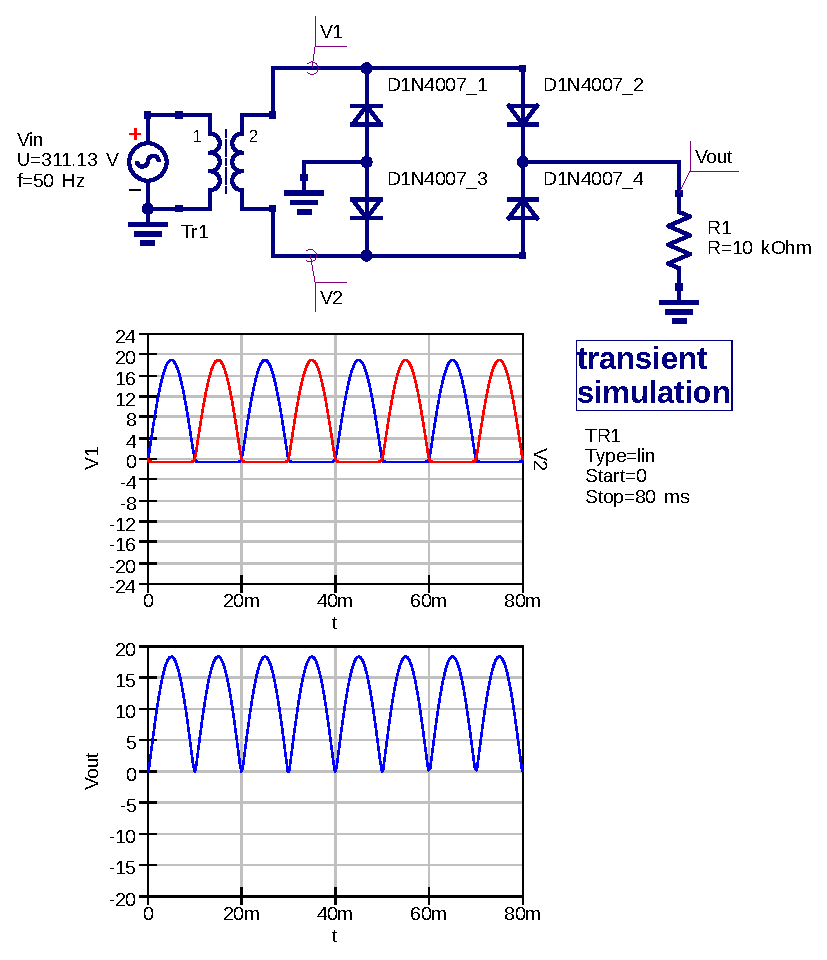
\includegraphics[scale=0.75]{simulacion/04.onda_completa1.eps}
\caption{Simulación del rectificador de onda completa con puente.}
\label{simulacion04}
\end{figure}

\subsubsection{Laboratorio}
Se presenta el rectificador de onda completa con puente armado en laboratorio y
su medición de voltaje de salida en la carga, en la
\textbf{figura~\ref{laboratorio06}}.

\begin{figure}[!h]
\centering
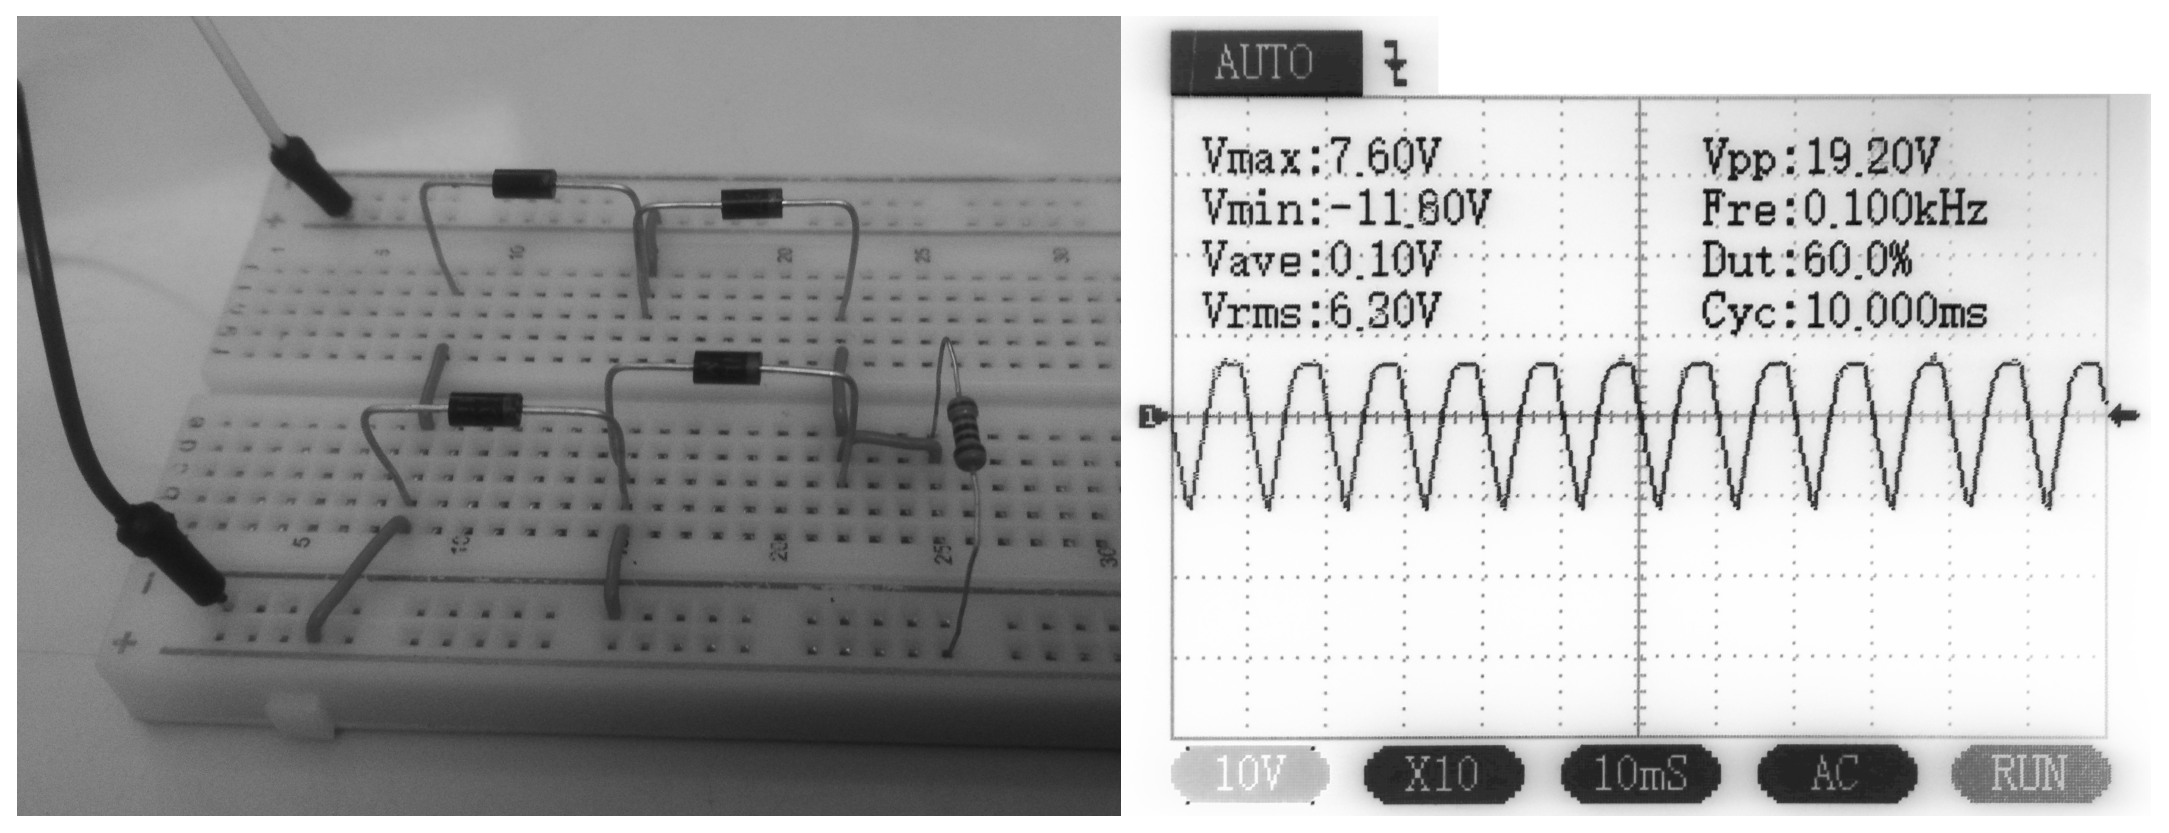
\includegraphics[scale=0.34]{fotos/04.onda_completa1.eps}
\caption{Rectificador de onda completa con puente.}
\label{laboratorio06}
\end{figure}

